\section{Introduction}
%%INTRODUCTION
%Describing the wider context: Introduce context & of your I&E Thesis. What is the context of you major thesis, your situation In your internship; your product/service offering or your focus area. In which part of the innovation process is your context currently in? Write down what has been done during the previous steps. Identify and discuss what should be done in the current and next steps (this can be short).

%Clear description of the context (internship, major thesis, start-up) to which the I&E minor thesis is linked

%Technical aspects of the context described in comprehensible way for non-experts
%Clear identification and statement of an I&E problem
%I&E problem well chosen, considering the available context

%Describing the wider context: Introduce context & of your I&E Thesis.
In the ever-changing market of online services, Cloud Computing played a vital role for the last decade. With the rise of \ac{IoT}, more and more machines/devices are getting connected to internet and more business opportunities are getting created. There are already many \ac{IoT} applications in the market and all of these services run in the cloud, as cloud provides scalability and fault tolerance. However, recent researches \citep{Fog, ciscowhite} has proved that to support \ac{IoT} application a different computing paradigm, namely Fog Computing has evolved. %We have envisioned a Fog Computing Solution which is under development.

%What is the context of you major thesis, your situation In your internship; your product/service offering or your focus area.
\subsection{Context}
I have been doing internship in Fraunhofer Institute for Open Communication Systems, also known as Fraunhofer FOKUS. In this institute, I have been working on the field of \ac{IoT}. We have envisioned a `Programmable Fog Node' solution which is a Fog Computing Solution. We have published a workshop paper\citep{ProgFogNode} about the envisage product. And currently we are developing this Fog Computing Solution.

Fog Computing is an alternative solution for running \ac{IoT} applications. As real Fog is like Cloud but stays near the ground. Similarly, Fog Computing \citep{Fog}, a term created by Cisco\footnote{Cisco Systems - \url{http://www.cisco.com/}}, is like Cloud Computing but near the sensor devices. According to Cisco, Fog extends cloud to be closer to the things that produce and act on IoT data\citep{ciscowhite}. In Fog Computing, any local computer with network connectivity can be a Fog node, host of the application server instead of Cloud datacenter. So, any  machine such as computer, router, switch that has computing capacity and can host \ac{IoT} application server can be a Fog node.


%Using OpenMTC anyone can develop \ac{IoT} application. And like all other \ac{IoT} application,  OpenMTC platform can receive sensor data or machine data and send the data to the applications running in the cloud. End-user can use the applications running in the cloud. All these features are common to \ac{IoT} applications and one example architecture is shown here in Figure~\ref{img:fog}.





% In which part of the innovation process is your context currently in? 

\subsection{Innovation and contribution}
Now-a-days there are many \ac{IoT} applications and services. Nearly all of them are running in the cloud. An example scenario is depicted in the Figure \ref{img:iotcloud} where in a smart home, \ac{IoT} applications are running in cloud data centers. Though Cloud computing is great for scalability and fault-tolerance, but for \ac{IoT} applications there are some limitations that cloud computing cannot address. 
%The problems will be discussed in the following sections. 
The major one is slow performance due to data travel to the cloud from the sensors. For example, imagine the smart home in the Figure \ref{img:iotcloud} has a motion sensor. When the owner leaves home, he can activate an alarm application. Later, if any intruder enters the home, the motion sensor can send that sensor data to the application server running in the cloud. The data is analyzed in the server and it generate an alarm to the owner's mobile application. All these data travel takes time. By the time the owner get the alarm, the intruder might leave. 

\begin{figure}[H]
  \centering
  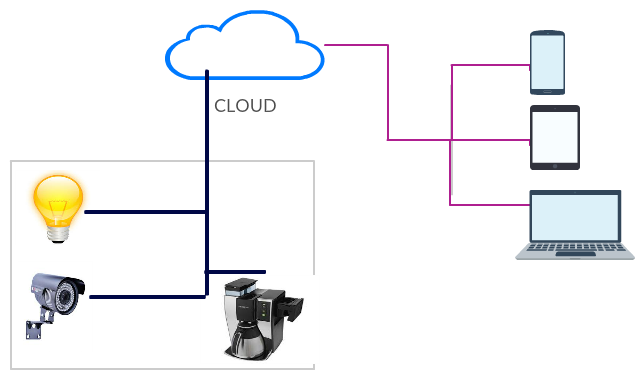
\includegraphics[width=.50\textwidth]{img/iot-cloud.png}
  \caption{Smart Home: IoT applications running in cloud}\label{img:iotcloud}
\end{figure}


As another example, in a smart industry if the temperature of an important machine is rising fast and a temperature sensor is monitoring that, immediate action, like shutdown, should be taken to avert costly failure. If the temperature sensor sends the data to the cloud where an application does the data analytics and send back a shutdown command to the machine, by the time the command reaches the machine, the opportunity to act on the machine might be gone. There are such cases where the \ac{IoT} application needs real-time performance for time-critical problems.

To address the problems for \ac{IoT} applications Fog computing emerged. As explained before, in Fog computing application server runs in Fog node near the devices, like that machine's temperature sensor or that motion sensor, instead of cloud. So, the data transfer from the sensor to application server in Fog node does not take time. The application server also sends back the data to machine or web/mobile application, faster than cloud. Thus, Fog computing improves performance and  overall \ac{QoS}. An example of Fog computing is shown in Figure \ref{img:iotfog} where in a smart home, \ac{IoT} applications are running in Fog nodes near the sensor devices and machines.

\begin{figure}[H]
  \centering
  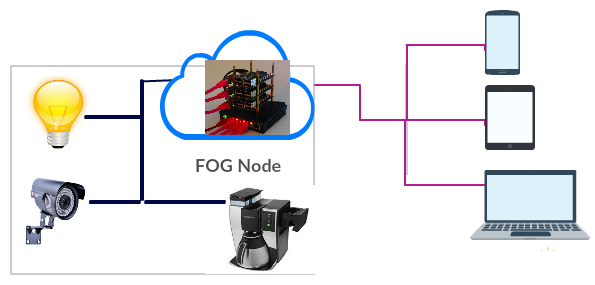
\includegraphics[width=.50\textwidth]{img/iot-fog.png}
  \caption{Smart Home: IoT applications running in Fog node}\label{img:iotfog}
\end{figure}

We are developing a `Programmable Fog Node' where anyone can host any kind of \ac{IoT} application. This can be a simple small computer that can run any \ac{IoT} application near the sensors.
%using Docker Container\footnote{Docker - \url{https://www.docker.com/}}. Docker Container, if used, takes away any dependency for running application in a host machine and can run any application on any machine which only docker installed. 

%Write down what has been done during the previous steps. Identify and discuss what should be done in the current and next steps (this can be short).
\subsection{Previous steps and future work}

So far we have conceptualized about the product and wrote a paper about our envisioned `Programmable Fog Node' which was accepted in a workshop \citep{ProgFogNode}. Currently, we are developing the product and we have a \ac{MVP}.

In this thesis, I tried to find out what features we should develop and add to our \ac{MVP} based on customer feedback. Future work includes developing these identified features and test them with users. 

%As soon as we have the prototype we will test it with users. Though there are several Fog computing solutions in the market, but our envisioned product differs clearly in many ways. Hosting the application in a seamless way using Docker container will be the major benefit of all. Still there will be scope to improve the services. In future application hosting in Fog node can be more advanced, like running multiple applications in a single Fog node using little computing power. We can also adapt our product with potential customers' feedback and requirements. 





%% Identifying your I&E problem or challenge in this context: Based on the above, please consider as part of the introduction short [in a few sentences], but precisely the following questions.
\subsection{I\&E Challenge}
%% What is the problem or challenge from an I&E perspective?

While we are developing a Fog Computing solution, there are few competitors who are already in the market like Cisco IOx\footnote{Cisco IOx - \url{https://developer.cisco.com/site/iox/}}, Prismtech's Vortex\footnote{Prismtech Vortex - \url{http://www.prismtech.com/vortex}}, Nebbiolo Fog node \footnote{Nebbiolo Fog node - \url{http://www.nebbiolo.tech/}}. %Though these products are pioneer, however they are in their early stage of marketing and hence there are not many customers for any solution. 

Machina Research estimates that there will be 12 billion \ac{M2M} connections globally in 2020, which was 2 billion in 2011 and Also 1.6 billion devices will be connected to fixed broadband\citep{machinareport}. So, potentially, Fog Computing solutions have a large market. Though the existing competitors provides effective Fog Computing solution, however they are in their early stage of marketing and hence no product has received notible customers yet. 

Since, we are still in the development phase we have the advantage to adapt our product to the customer need, even before we finish the development. Modifying our `Programmable Fog Node' by adding features that customer want, can give us the opportunity to receive many early adopters and develop best Fog Computing solution in the market. 
%We can use Design Thinking method.

%As we have been putting our effort to be in the market, we need to understand beforehand how much customer can we get in this market. And what features can differentiate us to meet more customer need and gain significant market share. 

%\subsubsection{Why it's I\&E challenge}

%% Why is this an important problem or challenge from an I&E perspective?
\ac{IoT} market, despite being predicted as an emerging market, is not expanding as expected. The Fog Computing solutions are said to be the future \citep{fogisfuture} of cloud computing for \ac{IoT} market. Yet, no Fog Computing solutions have gained notable customers. So, we feel that there are some probable gaps between the offered solutions and what customers' really want. That's why we think our challenge is not lying in the feasibility of the solution, rather in finding out what our customers' really need in our Fog Computing solution. We have nice features in our envisioned product, but before developing we want to learn if these features are something that customers want. According to Eric Ries, "additional features or polish beyond what early adopters demand is a form of wasted resources and time."\cite[p.~87]{leanstartup}. That's why we want to find out what our customers really need and then add the required features in our solution. %for the prototype we want to develop something that can help us to gain the early adopters. 


%If we fail to assess the customer need before we go into market, it can lead us to fail. 

%% What do you know about the problem or challenge?

%\subsubsection{What do you know about the problem or challenge?}

I know who are the potential users and customers for our product, which will help me to solve my I\&E problem. Our users are the people who will develop and run \ac{IoT} application in our Fog Computing solution. However, our customers are the people who will be benefited from running these applications in our Fog Computing solutions, e.g. industry owner, smart home owner, smart grid company etc. 
%The customers can be the industry owner who want to run \ac{IIoT} applications, smart home owners etc. 
%We can get the feedback from the users about our product. 
For this reason, I know to whom I should go to ask what features they want to see in our product. 
%If we follow any product design methods, like Design Thinking \citep{designthinkingIDEO} and Lean Startup \citep{leanstartup} we know the user-segments to verify our idea and know their requirements.

%As our product is still development phase, so we still have the opportunity to adjust our product and add features according to the customer need. we have been following lean start-up methodology to develop our product. So, the product is a prototype and there are some customers who bought the license. There are also some potential customers whom we can communicate to assess their need. 

%\subsubsection{What don’t you know about the problem or challenge?} 

However, we also need to consider our competitors. There are some big companies in this market, e.g. Cisco Systems. Though they have introduced Fog computing in their product, yet they are including more features in every life cycle. So, we don't know what additional features can they add in upcoming releases that can potentially challenge us more. But this is not in our hand, so we can try to figure out what feature customers need right now in order to bring best product for current market.

%Based on the 4 items above, formulate an Innovation or Entrepreneurial study or research question/challenge to be addressed in this I&E Thesis and which relates to either:
%%•Your major thesis (may be the wider focus area, or a hypothetic implementation of the technology)
%%•Your internship
%%•Another I&E problem experienced during your studies (be sure to show in this case, what the new aspects are that you address in this I&E thesis, that you had not addressed before. These should be significant!

%\subsection{Entrepreneurial Challenge for Us}

In this I\&E Thesis, I am going to find out, based on the existing theories and tools, how can I get feedback from the customer about what they need to develop the best product in the \ac{IoT} market. %There are established methodologies for these works, e.g. like Design Thinking \citep{designthinkingIDEO}, Lean Startup\citep{leanstartup}  Customer Development \citep{fstE}. 

The remainder of this thesis is structured as follows. In the next section, I reviewed the existing literatures and methods to get user feedback about a product. In following section 3, I discussed which methods I have followed to get user feedback. I also listed the findings from user feedback and how these findings helped me to solved my I\&E problem.

%Though, there are such tools and methods, we have to find out which one is best suitable for our use cases after an extensive literature review. When we will find a matching tool, we can use that tool to get customers' needs. Then we can develop according to their needs. 
















\begin{comment}

\ac{M2M} communication is increasing more and more, There has been projections that billions of devices will be connected by 2020. 

Introducing fog computing to OpenMTC will 

Introduction of cloud computing changes the way Web-applications works completely. Instead of hosting application in the in-house infrastructure, hosting application on remote datacenter (cloud) changed the cost of running application. In most cases, it's more cost effective to host application in cloud rather than setting up in-house infrastructure.

But, for \ac{M2M} applications, running application in cloud is not so efficient for number of reasons. 

Research institute like Machina research\footnote{Machine research -\url{https://machinaresearch.com/forecasts/main/}}  and Gartner\footnote{Gartner - \url{http://www.gartner.com/technology/home.jsp}} forecasts shows us more and more devices, machines will be connected to internet and they will be able to operate autonomously.

So, running machine-2-machine (M2M) applications in a internet
enabled local-computer will save data-bandwith which will reduce cost significantly and also increase application performance which will increase user experience, giving the m2m applications more acceptable. 
\end{comment}}





